\section{Methods}
We utilize genetic algorithms as our evolutionary simulation tools. The gene regulatory network that we used in this paper was originally proposed by Wagner \cite{wagner1996does} and customized by Espinosa-Soto and Wagner \cite{espinosa2010specialization} as well as Larson et al. \cite{larson2016recombination}. 

All simulation code was implemented in Java 1.8.0 and Python 2.7.10. They are all publicly available at https://github.com/xxxxxxxxxx. Modularity was evaluated using the NetworkX package with the community API \cite{hagberg2008exploring}. All the generated data can be downloaded at: https://drive.google.com/file/d/0B9dNEi7lDXnldy1sNmZuTWNXMDg/view?usp=sharing. 
\subsection{Model}
Cells in an organism display heterogeneity in functionalities and morphologies, while they contain the same set of genes. In other words, cells interpret the same genetic material in different ways so that their behaviors and structures vary. These distinct interpretations are due to the regulation via the activation and repression of genes \cite{wagner1996does}. In brief, effects of different genes are not mutually independent. A protein that is generated by a gene may activate or repress other genes. A gene regulatory network can be a mathematical directed graph to express these relationships of genes in an organism \cite{wagner1996does}. Specifically, genes can have two different patterns, namely activation and repression. The term "gene activity pattern" is adopted to represent the activeness status of the entire set of genes. Different gene activity patterns mean the distinct cellular functions and forms \cite{espinosa2010specialization}. 

We reconstructed the model that was utilized in the work done by Espinosa-Soto and Wagner, which is a model to represent a gene regulatory network \cite{espinosa2010specialization}. In this model, a gene regulatory network with $N$ genes will be in the form of an adjacency matrix $A = a_{ji}$, which acts as a genotype of an individual. Each entry $a_{ji}$ is restricted to be either 1, 0 or -1, which represents an activation, absence or repression interaction from gene $j$ to gene $i$, respectively. The gene activity pattern of this network at time $t$ can be expressed as a Boolean row vector $s_{t} = [s_{t}^0,...,s_{t}^{N-1}]$. A certain gene $i$ can either be active ($s_t^i=1$) or inactive ($s_t^i=-1$). The transition of state activity is modeled by the equation below
\begin{equation}
s_{t+\tau}=\sigma[\sum_{j=1}^{N}a_{ji}s_t^j]
\end{equation}
where $\sigma(x)$ equals 1 if $x>0$ and is 0 otherwise. 
\subsection{Fitness}
The fitness here evaluates the likelihood that an attractor is obtained when facing perturbations \cite{espinosa2010specialization}. In other words, Espinosa-Soto and Wagner imposed a bias of robustness on their gene regulatory network models in order to indirectly select modular networks. This is because modular networks can limit perturbations in a module so that the overall structure will not be heavily affected \cite{aderems2005systems}. That is, more modular networks are more robust. 

There are two or more stages in their experiments on discovering the conditions under which modularity starts emerging. In the first stage, gene regulatory networks are evolved under selective pressure towards regulating a particular gene activity pattern, while facing some perturbations. The original gene activity pattern before perturbation is called a target. In the second and further stages, networks are evolved under selective pressure to regulate new gene activity patterns, while preserving the ability to regulate the old patterns. In the particular case where there were two gene activity patterns, the first stage lasted for 500 generations and the second took another 1500 generations. 

The perturbations of targets are randomly generated in every generation when evaluating the fitness of gene regulatory networks. In Espinosa-Soto and Wagner's experiments, a network would face 500 perturbations comprising different corrupted versions of gene activity patterns. Each gene will have a probability of 0.15 to be perturbed into its opposite activity. A further study was conducted to explore a sufficient number of perturbations in order to shorten the computational time while maintaining a similar eventual improved modularity. It was concluded that 75 or 100 perturbations would lead to the noteworthy emergence of modularity \cite{totten2015exploring}. Therefore, 75 perturbations are undertaken for evaluating the fitness of each gene regulatory network in order to reduce the running time. 

Larson et al. applied another approach for evaluating the fitness of networks \cite{larson2016recombination}. They generated a static set of perturbations at the beginning and utilised this same set of corrupted targets whenever network fitness was calculated. This method converts the original stochastic fitness evaluation into a deterministic one. That is, the evolutionary landscape of individuals under this fitness evaluation will remain unchanged in each generation. On contrast, Espinosa-Soto and Wagner's fitness evaluation will lead to the evolutionary landscape to shift every generation. 

The fitness value of a gene regulatory network reflects its robustness in recovering from various perturbations. The error function compares an attractor of the network dynamics to the original gene activity pattern. That is, a successful network is able to regulate a corrupted pattern to its initial form. Then, the Hamming Distance G between the attractor and the original pattern was calculated. Previous experiments indicated that it normally took fewer than 20 transitions to reach the attractor \cite{wagner1996does}. Thus, non-stable attractors are assumed to be those gene regulatory networks that take more than 20 steps to attain the stability, or are cyclically stable. They are treated to have a maximum Hamming distance $D_{max}$. This is followed by a calculation of the contribution from each perturbation attractor to the fitness, which is defined as a developmental trajectory $\gamma=(1-D/D_{max})^5$ \cite{espinosa2010specialization}. Afterwards, this process is repeated to determine 75 $\gamma_{i}$, $1 \leq i \leq 75$. Finally, the fitness of a network is calculated as
\begin{equation}
f(g)=1-e^{-3g}
\end{equation}
where $g$ represents the arithmetic mean of the sum of all $\gamma_{i}$ \cite{espinosa2010specialization}. As to cases where there are more than one gene activity patterns, the arithmetic mean of $f(g)$ for all the patterns was take. Consequently, a gene regulatory network with a high fitness is able to lead to different attractors matching different targets. 
\subsection{Evolutionary Simulations}
Espinosa-Soto and Wagner imposed a bias towards low-density gene regulatory networks in mutation \cite{espinosa2010specialization}. A node in the network has a probability $\mu=0.05$ to mutate every generation, and it either can lose or gain an interaction. The probability for a node to lose an interaction can be calculated as
\begin{equation}
p(u)=\frac{4r_{u}}{4r_{u} + N - r_{u}}
\end{equation}
where $N$ is the number of gene nodes in a gene regulatory network, and $r_{u}$ equals to the number of regulators of gene $u$ \cite{espinosa2010specialization}. That is, the number of genes that exert effects on gene $u$. In contrast, the probability for a gene $u$ to obtain an interaction is defined to be $1-p(u)$. That is, it can keep the sparseness of the network, which computational biology research suggests is necessary for the emergence of modularity. 

Espinosa-Soto and Wagner did not apply a crossover mechanism in their simulation \cite{espinosa2010specialization}. In the reconstructed model by Larson et al., they limited crossover to nine possible partition locations of a 10-node network, corresponding to nine possible rows for splitting the adjacency matrix of a network horizontally \cite{larson2016recombination}. We call this horizontal crossover. When two matrices $A_{1}$ and $A_{2}$ are selected for crossover at index $i$, matrices of their children will be produced as \\ \\
$C_{1}[0: i-1, :] = A_{1}[0: i-1, :]\\
C_{1}[i: 9, :] = A_{2}[i: 9, :]\\
C_{2}[0: i-1, :] = A_{2}[0: i-1, :]\\
C_{2}[i: 9, :] = A_{1}[i: 9, :]\\$

However, this horizontal crossover may not only make the parental networks exchange modular clusters, but also exchange some interactions between the two modules. This may corrupt modularity. In contrast, we use a crossover mechanism that swaps interactions between modules in a gene regulatory network with connections between modules in another network. We refer this as diagonal crossover. Compared with the crossover mechanism of Larson et al., this approach, as Figure \ref{fig:diagnonal-crossover} illustrates, will better preserve the community structure (Wilcoxon signed-rank test; $p<0.0372$).
\begin{figure}[h!]
	\centering
	\begin{subfigure}[b]{0.4\linewidth}
		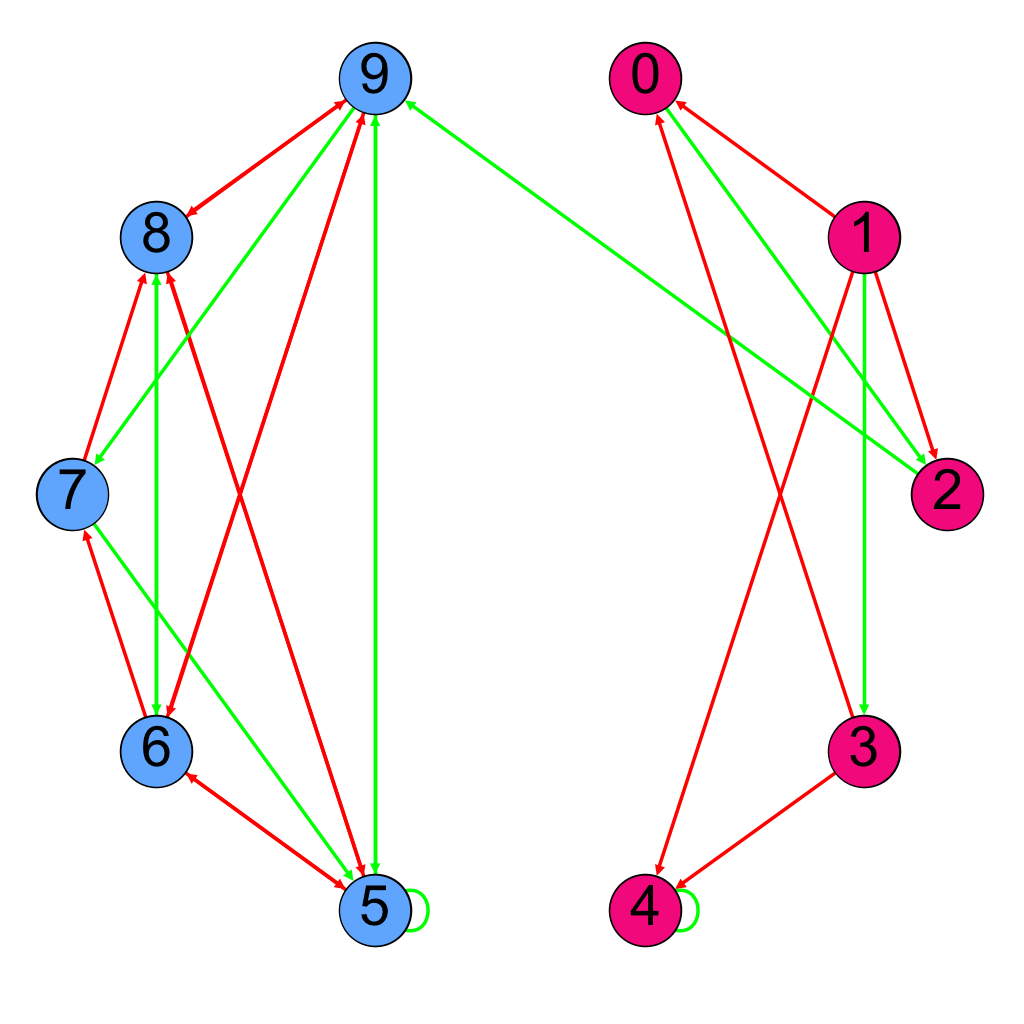
\includegraphics[width=\linewidth]{crossover-1.png}
		\caption{Parental network 1.}
	\end{subfigure}
	\begin{subfigure}[b]{0.4\linewidth}
		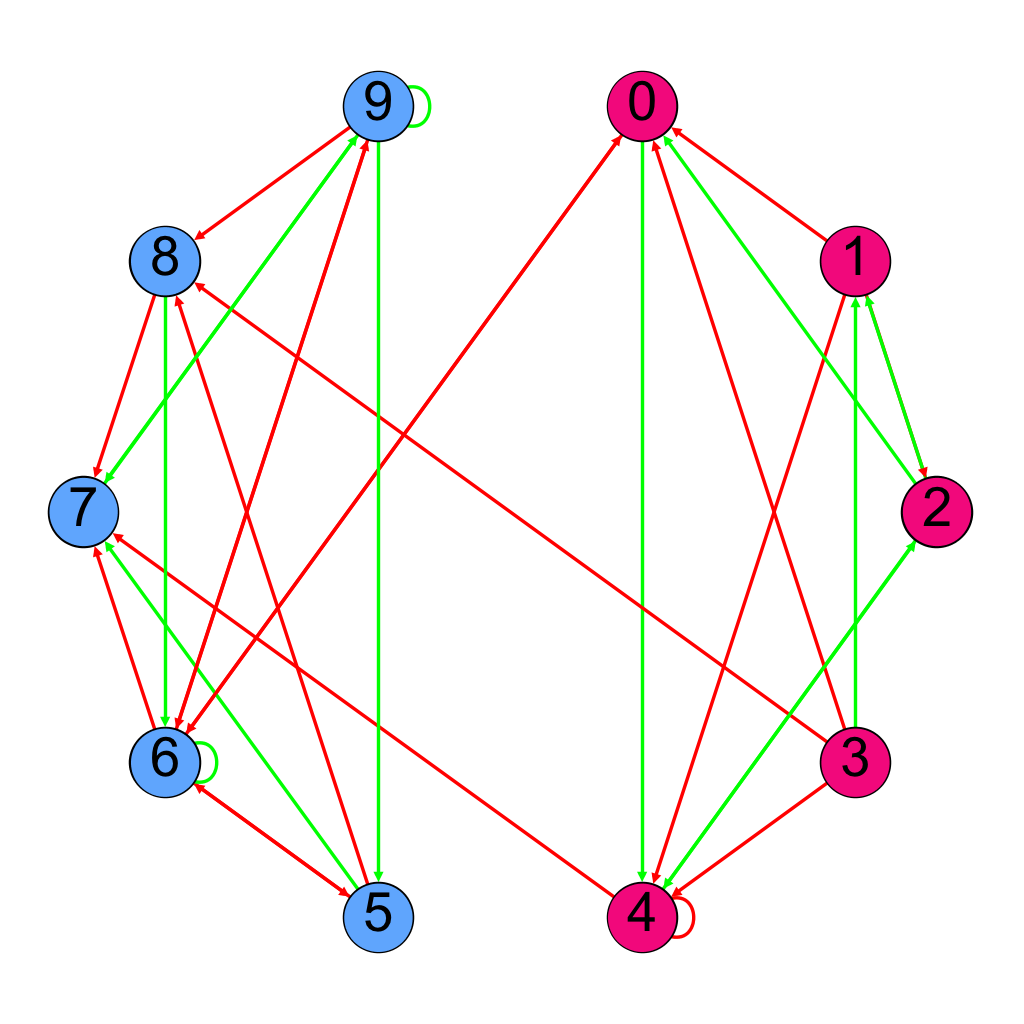
\includegraphics[width=\linewidth]{crossover-2.png}
		\caption{Parental network 2.}
	\end{subfigure}
	\begin{subfigure}[b]{0.4\linewidth}
		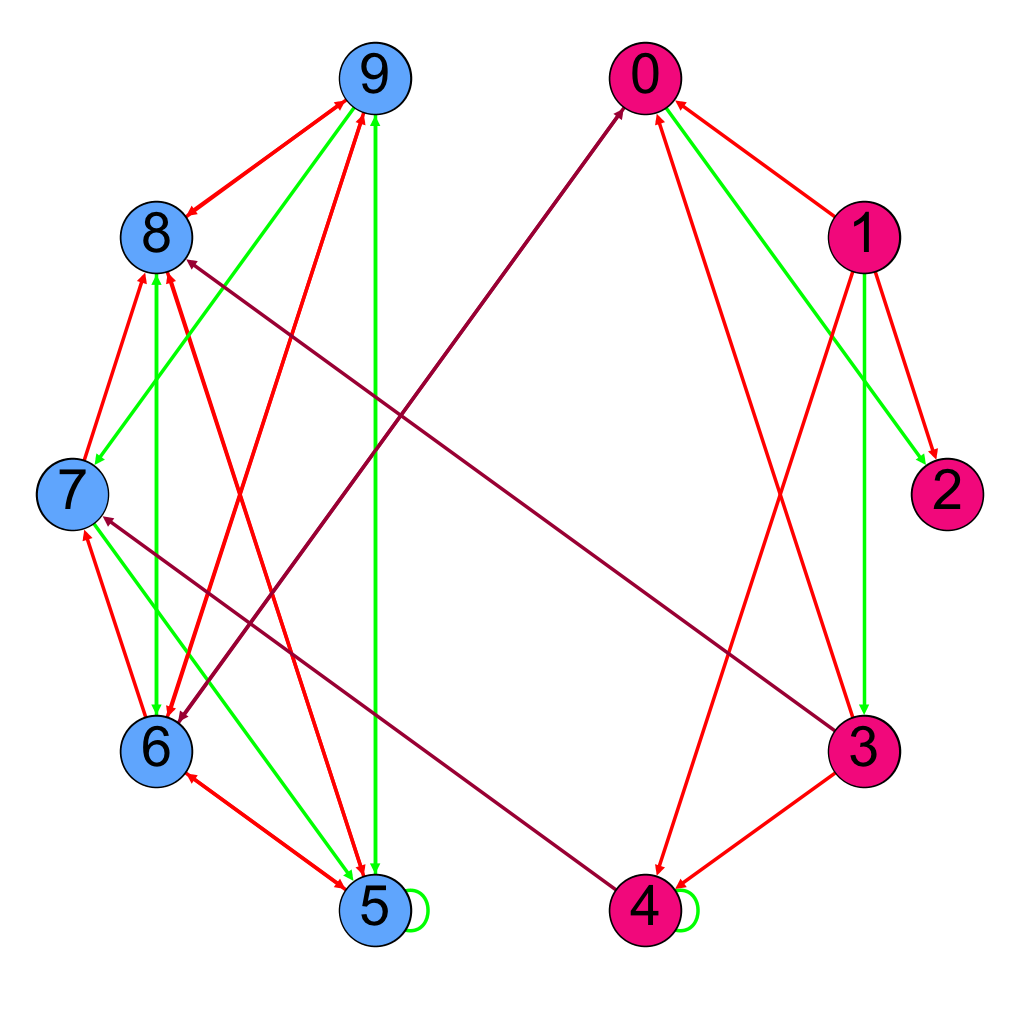
\includegraphics[width=\linewidth]{chin-crossover-1.png}
		\caption{Child network 1.}
	\end{subfigure}
	\begin{subfigure}[b]{0.4\linewidth}
		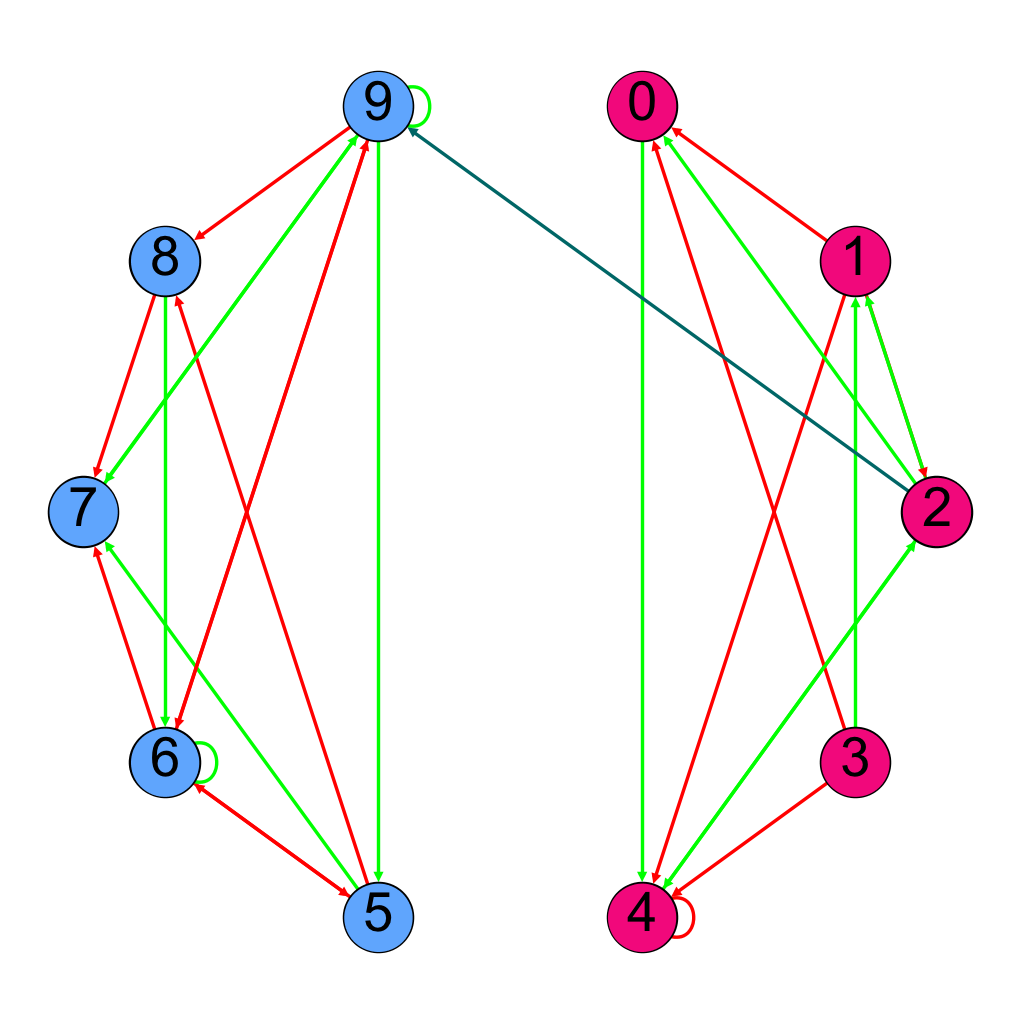
\includegraphics[width=\linewidth]{chin-crossover-2.png}
		\caption{Child network 2.}
	\end{subfigure}
	\caption{Demonstration of diagonal crossover}
	\label{fig:diagnonal-crossover}
\end{figure}
\subsection{Modularity Metric}
We adopted the Q scoring system to quantify modularity in a network based on the algorithm proposed by Newman \cite{newman2004finding}. Briefly, this approach is defined as the difference between the ratio of the number of edges in the network connecting nodes within a module over the number of all the edges, and the same quantity when assigning the nodes into the same modules yet edges are assumed to be randomly connected in the network \cite{kashtan2005spontaneous}. Formally, $Q$ is calculated as 
\begin{equation}
Q = \sum_{i}^{K}[\frac{l_i}{L} - (\frac{d_i}{2L})^2]
\end{equation}
where $i$ represents one of the $K$ potential modules within a network, $L$ is the total number of connections in a network, $l_i$ stands for the number of interactions in the module $i$, and $d_i$ is the sum of degrees of all the nodes in module $i$ \cite{espinosa2010specialization}. In other words, $Q$ considers the two ratios of both intra-module connection density and inter-module connection density \cite{newman2004finding}. A network that is considered to be good on modularity must consist of as many within-module edges and as few inter-module edges as possible. However, it will result in $Q=0$ if all the nodes are partitioned into the same module. 

The value $Q$ will sit in the range of $\left.[-\frac{1}{2}, 1\right.)$. Nodes in the gene regulatory network are partitioned into different groups according to their regulating gene activity patterns. 


